\documentclass[utf8]{article-hermes}
% Created by Y. Lepage 08/10/2012

% Merci de remplir
% la date de soumission : JJ/MM/AAAA
% le volume et le numéro de TAL auquel vous soumettez (p. ex. : 54-1) : VV-NN
% s'il s'agit de la première soumission (1) ou de la deuxième après premières
% relectures (2) : R

\usepackage{xifthen}
\usepackage{tikz}
\usepackage{booktabs}
\usepackage{rotating}
\usepackage{multirow}
\usepackage{amsmath}
\usepackage{varwidth}
\usepackage{overpic}
\usepackage{lipsum}
\usepackage{xfrac}
\usepackage{pgfplots}
\usepackage{url}
\usepackage{subfigure}
\usepackage{fancybox}
\usepackage{multicol}
\usepackage[inline]{enumitem}

\pgfplotsset{compat=1.8}

\usetikzlibrary{positioning, topaths, shapes, arrows, patterns}

\newcommand\newcite[2][]{\ifthenelse{\equal{#1}{}}{\citeasnoun{#2}}{\citeasnoun[#1]{#2}}}
\newcommand\TODO[1]{\textcolor{red}{[TODO #1]}}

\newtheorem{property}{Propriété}

%%%%%%%%%%%%%%%%%%%%%%%%%%%%%%%%%%%%%%%%%%%%%%%%%%%%%%%%%%%%%%%%%%%%%%%%%%%%%%%%

%\submitted[06/06/2014]{TAL~55-1}{R}
\journal{TAL. Volume 55 -- n° 1/2014}{45}{69}

\title[TopicRank]{TopicRank~: ordonnancement de sujets\\
                  pour l'extraction automatique\\
                  de termes-clés}

\author{Adrien Bougouin\fup{*} \andauthor\ Florian Boudin\fup{*}} 

\address{\fup{*} LINA - UMR CNRS 6241, Université de Nantes\\
         UFR de Sciences et Techniques, 2 rue de la Houssinière, 44322 Nantes,
         France\\
         \textit{prenom.nom}@univ-nantes.fr}

\resume{Les termes-clés sont les mots ou les expressions polylexicales qui
représentent le contenu principal d'un document. Ils sont utiles pour diverses
applications telles que l'indexation automatique ou le résumé automatique, mais
ne sont cependant pas disponibles pour la plupart des documents. La quantité de
ces documents étant de plus en plus importante, l'extraction manuelle des
termes-clés n'est pas envisageable et la tâche d'extraction automatique de
termes-clés suscite alors l'intérêt des chercheurs. Dans cet article nous
présentons \textit{Topic\-Rank}, une méthode non supervisée à base de graphe
pour l'extraction de termes-clés. Cette méthode groupe les termes-clés candidats
en sujets, ordonne les sujets et extrait de chacun des meilleurs sujets le
terme-clé candidat qui le représente le mieux. Les expériences réalisées
montrent une amélioration significative vis-à-vis de l'état de l'art des
méthodes à base de graphe pour l'extraction non supervisée de termes-clés.}
\abstract{Keyphrases are single or multi-word expressions that represent the
main content of a document. As keyphrases are useful in many applications such
as document indexing or text summarization, and also because the vast amount of
data available nowadays cannot be manually annotated, the task of automatically
extracting keyphrases has attracted considerable attention. In this article we
present TopicRank, an unsupervised graph-based method for keyphrase extraction.
This method clusters the keyphrase candidates into topics, ranks these topics
and extracts the most representative candidate for each of the best topics. Our
experiments show a significant improvement over the state-of-the-art graph-based
methods for keyphrase extraction.}
\motscles{extraction de termes-clés, groupement en sujets, ordonnancement de
sujets, méthode non supervisée, méthode à base de graphe.}
\keywords{keyphrase extraction, topic clustering, topic ranking, unsupervised
method, graph-based method.}

%\date{}
\begin{document}

\maketitlepage

\section{Introduction}
\label{sec:introduction}
  % * définition de terme-clé, applications et enjeux
  Un terme-clé est un mot ou une expression polylexicale qui représente un
  concept important d'un document auquel il est associé. En pratique, plusieurs
  termes-clés représentant des concepts différents sont associés à un même
  document. Ils forment alors un ensemble de termes-clés à partir duquel il est
  possible de déduire le contenu principal du document. Du fait de leur capacité
  à synthétiser le contenu d'un document, les termes-clés sont utilisés dans
  diverses applications en Recherche d'Information (RI)~: résumé
  automatique~\cite{avanzo2005keyphrase}, classification de
  documents~\cite{han2007webdocumentclustering}, indexation
  automatique~\cite{medelyan2008smalltrainingset}, etc. Avec l'essor du
  numérique, de plus en plus de documents (articles scientifiques, articles
  journalistiques, etc.) sont accessibles depuis des médiums d'informations tels
  que Internet. Afin de permettre à un utilisateur de rapidement trouver des
  documents, ainsi que d'avoir un bref aperçu de leur contenu, les tâches
  sus-mentionnées sont nécessaires.
  Cependant, la majorité des documents ne sont pas associés avec des termes-clés
  et, compte tenu du nombre important de documents numériques, l'ajout manuel de
  ces derniers n'est pas envisageable. Pour pallier ce problème, de plus en plus
  de chercheurs s'intéressent à l'extraction automatique de termes-clés et
  certaines campagnes d'évaluations, telles que DEFT~\cite{paroubek2012deft} et
  SemEval~\cite{kim2010semeval}, proposent des tâches d'extraction automatique
  de termes-clés.

  % * qu'est-ce que l'extraction automatique de termes-clés
  % * deux écoles : indexation libre et indexation contrôlée (assignation de
  %                 termes-clés)
  %   -> nous sommes de la première école
  % * deux catégories de méthodes : supervisées et non-supervisées
  %    -> en supervisé ils utilisent la structure des documents
  %    -> très peu de travaux en non-supervisé (filtrage des candidats)
  L'extraction automatique de termes-clés, ou indexation libre, est la tâche qui
  consiste à extraire les unités textuelles les plus importantes d'un document,
  en opposition à la tâche d'assignation automatique de termes-clés, ou
  indexation contrôlée, qui consiste à assigner des termes-clés à partir d'une
  terminologie donnée~\cite{paroubek2012deft}. Parmi les méthodes d'extraction
  automatique de termes-clés existantes, nous distinguons deux catégories~: les
  méthodes supervisées et les méthodes non-supervisées. Dans le cas supervisé,
  la tâche d'extraction de termes-clés est considérée comme une tâche de
  classification binaire~\cite{witten1999kea}, où il s'agit d'attribuer la
  classe \og{}\textit{terme-clé}\fg{} ou \og{}\textit{non terme-clé}\fg{} aux
  termes-clés candidats extraits du document. Une collection de documents
  annotés en termes-clés est alors nécessaire pour l'apprentissage d'un modèle
  de classification reposant sur divers traits, allant de la simple fréquence
  aux informations structurelles du document (titre, résumé, introduction,
  conclusion, etc.). Dans le cas non-supervisé, les méthodes attribuent un
  score d'importance à chaque candidat en fonction de divers indicateurs tels
  que la fréquence et la position de la première occurrence dans le document.
  Bien que les méthodes supervisées soient en général plus performantes, la
  faible quantité de documents annotés en termes-clés disponibles, ainsi que la
  forte dépendance des modèles de classification au type des documents à partir
  desquels ils sont appris, poussent les chercheurs à s'intéresser de plus en
  plus aux méthodes non-supervisées.

  % * ici, on cherche à identifier l'échelle de difficulté d'indexation des
  %   documents en Sciences Humaines et Sociales (SHS)
  % * on dispose de 4 collections de notices de 4 disciplines différentes de
  %   SHS + 1 collection de notices de chimie (science dure)
  Dans cette article, nous nous intéressons à l'extraction non-supervisée de
  termes-clés dans les articles scientifiques, et plus particulièrement à la
  performance des méthodes d'extraction de termes-clés dans des domaines de
  spécialité. Au moyen de cinq corpus disciplinaires, notre objectif est
  d'observer et d'analyser l'échelle de difficulté pour l'extraction
  automatique de termes-clés dans des articles scientifiques appartenant à cinq
  disciplines différentes~: Archéologie, Sciences de l'Information,
  Linguistique, Psychologie et Chimie.
  \TODO{Dire pourquoi nous nous intéressons aux méthodes non-supervisées}
  \TODO{Dire pourquoi nous nous intéressons aux articles scientifiques}

  % * annonce du plan
  L'article est structuré comme suit. Un bref état de l'art est donné dans la
  section~\ref{sec:etat_de_l_art}, les données utilisées sont présentées dans la
  section~\ref{sec:presentation_des_donnees} et les expériences menées, ainsi
  que les résultats obtenus, sont décrits dans la section~\ref{sec:experiences}.
  Enfin, une analyse des résultats est donnée dans la
  section~\ref{sec:discussion}, puis une conclusion générale et des perspectives
  de travaux futurs sont présentés en
  section~\ref{sec:conclusion_et_perspectives}.


\section{État de l'art}
\label{sec:etat_de_l_art}
  % Quel est le fonctionnement général des méthodes d'extraction automatique de
  % termes-clés ?
  L'extraction automatique de termes-clés est une tâche répartie en quatre
  étapes. Les documents sont considérés un par un, ils sont tout d'abord
  enrichis linguistiquement (segmentés en phrases, segmentés en mots, étiquetés
  en parties du discours, etc.), puis des termes-clés candidats en sont extraits
  et classifiés, ou ordonnés, afin de pouvoir sélectionner leurs termes-clés
  (cf. figure~\ref{fig:etapes_de_l_extraction_de_termes_cles}). L'extraction des
  termes-clés candidats et leur classification, ou ordonnancement, sont les deux
  étapes auxquels nous nous intéressons dans cet article. En effet, la
  classification, ou l'ordonnancement, des termes-clés candidats est le c\oe{}ur
  de la tâche d'extraction de termes-clés, mais ses performances dépendent de la
  qualité des candidats préalablement extraits.
  \begin{figure}
    \tikzstyle{io}=[
      ellipse,
      minimum width=5cm,
      minimum height=2cm,
      fill=green!20,
      draw=green!33,
      transform shape,
      font={\huge}
    ]
    \tikzstyle{component}=[
      text centered,
      thick,
      rectangle,
      minimum width=11cm,
      minimum height=2.5cm,
      fill=cyan!20,
      draw=cyan!33,
      transform shape,
      font={\huge\bfseries}
    ]

    \centering
    \begin{tikzpicture}[thin,
                        align=center,
                        scale=.45,
                        node distance=2cm,
                        every node/.style={text centered, transform shape}]
      \node[io] (document) {document};
      \node[component] (preprocessing) [right=of document] {Prétraitement Linguistique};
      \node[component] (candidate_extraction) [below=of preprocessing] {Extraction des candidats};
      \node[component] (candidate_classification_and_ranking) [below=of candidate_extraction] {
        \begin{tabular}{r|lcl}
          Classification & des candidats\\
          Ordonnancement &\\
        \end{tabular}
      };
      \node[component] (keyphrase_selection) [below=of candidate_classification_and_ranking] {Sélection des termes-clés};
      \node[io] (keyphrases) [right=of keyphrase_selection] {termes-clés};

      \path[->, thick] (document) edge (preprocessing);
      \path[->, thick] (preprocessing) edge (candidate_extraction);
      \path[->, thick] (candidate_extraction) edge (candidate_classification_and_ranking);
      \path[->, thick] (candidate_classification_and_ranking) edge (keyphrase_selection);
      \path[->, thick] (keyphrase_selection) edge (keyphrases);
    \end{tikzpicture}
    \caption{Les quatre principales étapes de l'extraction automatique de
             termes-clés. \label{fig:etapes_de_l_extraction_de_termes_cles}}
  \end{figure}

  \subsection{Extraction de termes-clés candidats}
  \label{subsec:extraction_de_termes_cles_candidats}
    % Quel est l'objectif ?
    L'objectif de l'extraction de termes-clés candidats est de réduire l'espace
    des solutions possibles aux seules unités textuelles ayant des
    particularités semblables à celles des termes-clés (tels qu'ils peuvent être
    donnés par des humains). Deux avantages directs à cela sont la réduction du
    temps de calcul nécessaire et la suppression d'unités textuelles non
    pertinentes pouvant engendrer du bruit affectant les performances de
    l'extraction de termes-clés. Pour distinguer les différents candidats
    extraits, nous définissons deux catégories~: les candidats positifs, qui
    sont de réels termes-clés, et les candidats non positifs, qui ne sont pas de
    réels termes-clés. Parmi les candidats non positifs, nous distinguons aussi
    deux catégories~: les candidats porteurs d'informations utiles à la
    promotions de candidats positifs et les candidats non pertinents, qui sont
    considérés comme des erreurs d'extraction.

    % Quels sont les différentes méthodes utilisées pour extraire les
    % termes-clés candidats ?
    Dans les travaux précédents pour l'extraction automatique de termes-clés,
    trois méthodes d'extraction de candidats sont classiquement utilisées~:
    l'extraction de n-grammes filtrés avec une liste de mots outils,
    l'extraction d'unités minimales de sens ayant pour tête un nom (chunks
    nominaux) ou l'extraction des unités textuelles respectant certains patrons
    syntaxiques.

    \subsubsection{Méthodes utilisées}
    \label{subsubsec:methodes_explorees}

      L'extraction de n-grammes consiste en l'extraction de séquences ordonnées
      de $n$ mots. Cette extraction est très exhaustive, elle fournit une grande
      quantité de termes-clés candidats, maximisant ainsi la quantité de
      candidats positifs ou porteurs d'informations, mais aussi la quantité de
      candidats non pertinents. Pour supprimer un grand nombre de ces candidats
      non pertinents, il est courant d'utiliser une liste de mots outils
      (conjonctions, prépositions, mots usuels, etc.). Une unité textuelle
      contenant un mot outils au début ou à la fin ne doit pas être considérée
      comme un terme-clé candidat. Bien que l'extraction de n-grammes filtrés
      fournisse un ensemble bruité de candidats, elle est encore largement
      utilisée dans les méthodes supervisées d'extraction automatique de
      termes-clés~\cite{witten1999kea,turney1999learningalgorithms,hulth2003keywordextraction}.
      En effet, du fait de leur phase d'apprentissage, les méthodes
      non-supervisées sont très robustes et donc peu sensibles aux bruits.

      L'extraction de chunks nominaux consiste en l'extraction d'unités
      minimales de sens ayant pour tête un nom. Contrairement aux n-grammes, les
      chunks sont toujours des unités textuelles grammaticalement correctes. De
      ce fait, elles sont moins arbitraires. D'un point de vue linguistique,
      l'extraction de chunks nominaux est plus justifiée que l'extraction de
      n-grammes. Cependant, son caractère plus restrictif ne permet pas
      d'extraire autant de candidats positifs. Il est donc important de
      s'assurer que les propriétés des chunks nominaux sont en accord avec les
      propriétés des termes-clés (tels qu'ils peuvent être donnés par des
      humains). Les expériences mennées par \newcite{hulth2003keywordextraction}
      et \newcite{eichler2010keywe} avec les chunks nominaux montrent une
      amélioration des performances vis-à-vis de l'usage de n-grammes.
      Cependant, \newcite{hulth2003keywordextraction} montre aussi qu'en tirant
      partie de l'étiquetage en parties du discours, l'extraction de termes-clés
      à partir de n-grammes donne des performances au-dessus de celles obtenues
      avec les chunks nominaux.

      L'extraction d'unités textuelles respectant certains patrons syntaxiques
      permet l'extraction de candidats qui sont grammaticalement et
      syntaxiquement contrôlés\footnote{Il est possible d'extraire les
      chunks nominaux à partir de patrons syntaxiques.}. Alors que
      \newcite{hulth2003keywordextraction} extraient des candidats avec les
      patrons de termes-clés les plus fréquents (plus de 10 occurrences) dans
      une collection de documents annotés, d'autres chercheurs tels que
      \newcite{wan2008expandrank} se concentrent uniquement sur les plus longues
      séquences de nom (nom propres inclus) et d'adjectifs.

      % Que veut-on apporter ?
      Dans le but d'améliorer la qualité des candidats extraits avec les
      méthodes susmentionnées, \newcite{kim2009termextraction} proposent de
      filtrer les candidats en fonction de leur spécificité vis-à-vis du domaine
      du document analysé. Cette spécificité est déterminée en fonction du
      rapport entre la fréquence d'un candidat dans le document et le nombre de
      documents dans lesquels il est présent \cite[TF-IDF]{jones1972tfidf}.
      Intuitivement, un candidat très fréquent dans le document analysé est
      d'autant plus spécifique à celui-ci s'il est présent dans très peu
      d'autres documents.

    \subsubsection{Méthodes pouvant être utilisées}
    \label{subsubsec:methodes_pouvant_etre_utilisees}
    
      L'idée de \newcite{kim2009termextraction} d'extraire des candidats
      spécifiques est une idée intéressant qu'il nous est possible d'étendre à
      l'usage de méthodes d'extraction terminologique. Les méthodes automatiques
      d'extraction terminologique, dont
      \newcite{castellvi2001automatictermdetection} en font la revue, extraient
      des mots ou expressions symbolisant un concept et devant, à ce titre,
      faire partie des entrées d'un index terminologique.

      Le système TermSuite\footnote{\url{http://www.ttc-project.eu}} est un
      outils état de l'art pour l'extraction terminologique monolingue et
      bilingue. Il combine à la fois le savoir linguistique et des statistiques
      calculées dans une collection de documents de spécialité (d'un domaine
      particulier), afin d'extraire les termes et leurs variantes (fautes
      d'orthographe incluses).

      En recherche d'information, \newcite{evans1996nounphraseanalysis} font le
      constat que les unités textuelles décrivant le mieux le contenu d'un
      document, et donc permettant de mieux l'indexer, sont majoritairement des
      termes. Ils proposent alors une méthode qui extrait dans un premier temps
      les groupes nominaux d'un document, puis en extrait les sous-composants.
      Ils définissent trois types distincts de sous-composants~:
      \begin{itemize}
        \item{les collocations~;}
        \item{les couples tête-modifieur~;}
        \item{les variantes des groupes prépositionnels.}
      \end{itemize}
      Dans le cas de l'extraction automatique de termes-clés, seuls les
      sous-composants étant présents dans le document analysé peuvent être
      extraits. Dans notre cas, il n'est donc pas toujours possible d'utiliser
      les couples tête-modifieurs et les variantes des groupes prépositionnels.

  \subsection{Classification/Ordonnancement des termes-clés candidats}
  \label{subsec:classification_ordonnancement_des_termes_cles_candidats}
    % Quel est l'objectif ?
    L'étape de classification/ordonnancement intervient après l'extraction des
    termes-clés candidats. Son rôle est de déterminer quels sont, parmi les
    candidats, les termes-clés du document analysé. La classification est
    majoritairement utilisée par les méthodes supervisées. Les méthodes
    non-supervisées, quant à elles,  effectuent en général un ordonnancement des
    candidats. Dans cet article, nous nous intéressons aux méthodes
    non-supervisées, nous ne présentons donc que ces dernières. De plus, les
    différences notables entre les différentes méthodes supervisées ne sont que
    dans le choix du classifieur (classifieur naïf bayésien, arbres de
    décisions, perceptron multi-couches, etc) ou des traits (TF-IDF, première
    position, parties du discours, etc.).

    % Quels sont les différentes méthodes non-supervisées existantes pour
    % l'extraction de termes-clés ?
    % Quels sont les inconvénients des méthodes actuelles ?
    % Que veut-on apporter ?
    Les méthodes non-supervisées d'extraction automatique de termes-clés
    emploient des méthodes très différentes, allant du simple usage de mesures
    statistiques~\cite{jones1972tfidf,paukkeri2010likey} au groupement des mots
    par fréquence de co-occurrences~\cite{liu2009keycluster}, en passant par
    l'utilisation de modèles de langues obtenus à partir de données
    non-annotées~\cite{tomokiyo2003languagemodel}, ou encore la construction
    d'un graphe de co-occurrences~\cite{mihalcea2004textrank}. Bien que dans la
    méthode que nous proposons nous faisons aussi du groupement, celle-ci
    appartient à la dernière catégorie de méthodes mentionnée. Nous nous
    intéressons donc, ici, aux méthodes dites \og à base de graphe~\fg.

    \newcite{mihalcea2004textrank} proposent une méthode d'ordonnancement
    d'unités textuelles à partir d'un graphe. Leur méthode, utilisée pour le
    résumé automatique et l'extraction de termes-clés, s'inspire de la méthode
    PageRank~\cite{brin1998pagerank} qui détermine l'importance d'une page Web
    grâce aux autres pages Web qui s'y réfèrent, ainsi qu'aux autres pages Web
    auxquelles elle se réfère. Le plus une pages Web est citée dans des pages
    Web différentes, le plus elle est importante, et le plus elle est
    importante, le plus elle donne d'importance aux pages Web auxquelles elle
    fait référence. Cette notion de référence entre les pages Web est
    représentée par un graphe dans lequel les n\oe{}uds sont des pages Web et
    les références les liens entre elles. Ensuite, une mesure de centralité,
    inspirée de la mesure de centralité eigenvector, est appliquée pour ordonner
    les pages Web par importance. Pour l'extraction de termes-clés avec TextRank
    les pages Web sont remplacées par les mots (nom et adjectifs) du document
    analysé et les liens entre eux symbolisent leur(s) co-occurrence(s) dans une
    fenêtre de $2$ mots. L'étape finale de la méthode consiste à générer les
    termes-clés à partir des $k$ mots les plus importants, les mots-clés. Les
    mots-clés sont marqués dans le documents et les plus longues séquences de
    mots-clés adjacents sont extraits comme termes-clés.

    \newcite{wan2008expandrank} proposent SingleRank. Cette méthode présente
    deux améliorations à TextRank. La première amélioration étend l'usage de la
    co-occurrence comme lien entre les mots et la seconde remplace l'étape de
    génération des termes-clés. Dans un premier temps, les auteurs pondèrent les
    liens de co-occurrence par leur nombre de co-occurrences calculées avec une
    fenêtres de $10$ mots. Ainsi un mot co-occurrent deux fois avec un autre est
    relié à celui-ci par un poids de $2$. Ce poids est ensuite utilisé pour
    transférer plus ou moins d'importance lors de l'ordonnancement.
    %Ce nouvel ordonnancement utilise plus d'informations présentes dans le
    %document analysé et est dotant plus efficace quand le document analysé est
    %de grande taille.
    L'importance ainsi calculée pour chaque mots est maintenant utilisée
    pour donner un score aux termes-clés candidats et ainsi les ordonner.
    Celui-ci est calculé en faisant la somme du score d'importance de chacun des
    mots qui le compose. Bien que la méthode SingleRank donne, dans la majorité
    des cas, des résultats meilleurs que ceux de TextRank, faire la somme du
    score d'importance des mots pour ordonner les candidats est une approche
    maladroite. En effet, cela a pour effet de faire monter dans le classement
    des candidats qui se recouvrent. Ainsi, dans le document
    \textit{as\_2002\_000700ar} de la collection DEFT (présentée dans la
    section~\ref{subsec:corpus_pour_l_extraction_de_termes_cles}) le candidat
    positif \og bio-politique~\fg\ est classé neuvième, alors que les autres
    candidats contenant \og bio-politique~\fg\ plus d'autres mots non
    nécessairement importants occupent les classements $2$ à $8$. Dans nos
    travaux nous ordonnons les termes-clés candidats en tenant compte de
    l'importance du sujet qu'ils représentent puis choisissons un représentant
    par sujet, nous évitons ainsi le problème rencontré avec SingleRank.

    Toujours dans l'optique d'utiliser plus d'informations pour améliorer
    l'efficacité de l'ordonnancement, \newcite{wan2008expandrank} étendent
    SingleRank en utilisant des documents similaires (documents voisins) au
    document en cours d'analyse. Leur approche consiste à observer les
    co-occurrences dans les documents voisins pour renforcer ou ajouter des
    liens dans le graphe initial. Cependant, en fonction de la similarité entre
    un document voisin et le document en cours d'analyse, des liens non
    pertinents risques d'être ajoutés. Pour y remédier, les auteurs utilisent le
    score de similarité entre les deux documents comme facteur d'atténuation de
    l'ajout ou du renforcement de liens. Cette approche donne des résultats au
    delà de ceux de SingleRank, mais il est important de noter que ses
    performances sont fortement liées à la possession de documents du même
    domaine que les documents analysés.

    A l'instar de \newcite{wan2008expandrank},
    \newcite{tsatsaronis2010semanticrank} tentent d'améliorer TextRank en
    modifiant le processus de création des liens entre les n\oe{}uds (mots) du
    graphe. Dans leur approche, un lien entre deux mots est créé et pondéré en
    fonction du lien sémantique de ces derniers selon
    WordNet~\cite{miller1995wordnet} ou
    Wikipedia~\cite{milne2008wikipediasemanticrelatedness}. Les expériences
    menées par les auteurs ne montrent pas d'amélioration vis-à-vis de TextRank.
    Ils montrent toute fois que l'ajout de connaissances lors de
    l'ordonnancement -- en biaisant l'ordonnancement en faveur des mots
    apparaissant dans le titre du document analysé ou en ajoutant le TFIDF dans
    le calcul du score d'importance -- améliore les résultats de sorte que
    ceux-ci soient au-dessus de ceux de TextRank.

    L'usage de sujets dans le processus d'ordonnancement avec TextRank est
    proposé par \newcite{liu2010topicalpagerank}. Reposant sur un modèle
    LDA~\cite[Latent Dirichlet Allocation]{blei2003lda}, leur méthode effectue
    un ordonnancement particulier pour chaque sujet, puis fusionne les rangs des
    mots pour chacun de ces ordonnancements, afin d'obtenir un ordonnancement
    global. L'ordonnancement en fonction de chaque sujet est biaisé par la
    probabilité de trouver un mot donné sachant ce sujet. Dan notre travail,
    nous émettons aussi l'hypothèse que le sujet auquel appartient une unité
    textuelle doit jouer un rôle majeur dans le processus d'ordonnancement.
    Cependant, nous tentons de nous abstraire de tout usage de documents
    supplémentaires et n'utilisons donc pas le modèle LDA. De même, il nous
    semble plus judicieux d'effectuer un seule ordonnancement, en prenant
    directement en compte l'appartenance d'une unité textuelle à un sujet
    particulier.


%\section{Présentation et analyse des données}
\label{sec:presentation_et_analyse_des_donnees}
  \subsection{Corpus pour l'extraction de termes-clés}
  \label{subsec:corpus_pour_l_extraction_de_termes_cles}

  \subsection{Termes-clés de référence}
  \label{subsec:termes_cles_de_reference}
    \begin{itemize}
      \item{présentation des statistiques}
      \item{proprietes observees}
      \item{quelles sont les méthodes d'extraction de candidats le plus en accord avec ces propriétés}
    \end{itemize}


\section{Extraction de termes-clés avec TopicRank}
\label{sec:extraction_de_termes_cles_avec_topicrank}
  \begin{itemize}
    \item{principe général}
    \item{identification des sujets}
    \item{ordonancement des sujets}
    \begin{itemize}
      \item{construction du graphe de sujets}
      \item{ordonnancement dans le graphe de sujets}
    \end{itemize}
    \item{selection des termes-clés}
  \end{itemize}


\section{Experimental Settings}
\label{sec:experimental_settings}
  \subsection{Dataset}
  \label{subsec:dataset}
    In this work, we use the SemEval corpus. Built for the task 5 of
    SemEval-2010~\cite{kim2010semeval}, Sem\-Eval contains 244 English
    scientific papers collected from the ACM Digital Libraries. We use
    Sem\-Eval's training set (144 documents) and test set (100 documents) with
    their sets of combined author- and reader-assigned keyphrases.

  \subsection{Baselines}
  \label{subsec:baselines}
    In order to show that our method benefits from all aspects of its
    configuration, we design a set of baselines that slightly diverge from our
    method (deried baselines). First, To\-picRank plus the SVM classifier
    trained on either topically independent and dependent features
    (TopicRank+SVM), while the SVM classifier is trained on all features for our
    method (TopicRank+SVM$_{all}$). Second the SVM classifier, trained on either
    topically independent, dependent or all features, is applied to the unranked
    clusters (Clustering+SVM). Finally, the SVM classifier, trained on topically
    independent features, is applied candidate keyphrases (SVM).

    For comparison purpose, we also report results of a Naive Bayes classifier
    trained with the first position and the TF-IDF
    features~\cite[KEA]{witten1999kea}, TF-IDF and TopicRank.

  \subsection{Preprocessing}
  \label{subsec:preprocessing}
%    For each document, we apply the following preprocessing steps: sentence
%    segmentation, word tokenization and Part-of-Speech tagging. For sentence
%    segmentation, we use the PunktSentenceTokenizer provided by the Python
%    Natural Language ToolKit~\cite[NLTK]{bird2009nltk}. For word tokenization,
%    we use the NLTK TreebankWordTokenizer for English and the Bonsai word
%    tokenizer\footnote{The Bonsai word tokenizer is a tool provided with the
%    Bonsai PCFG-LA parser:
%    \url{http://alpage.inria.fr/statgram/frdep/fr_stat_dep_parsing.html}.} for
%    French. As for Part-of-Speech tagging, we use the Stanford POS
%    tagger~\cite{toutanova2003stanfordpostagger} for English and
%    MElt~\cite{denis2009melt} for French.
    %%%%%%%%%%%%%%%%%%%%%%%%%%%%%%%%%%%%%%%%%%%%%%%%%%%%%%%%%%%%%%%%%%%%%%%%%%%%
    For our method, as well as all baselines, we use Topic\-Rank's outputs.
    Therefore, our results can directly be compared to results
    in~\cite{bougouin2013topicrank}.

  \subsection{Evaluation Measures}
  \label{subsec:evaluation_measures}
    We evaluate the performances of our method and the baselines in terms of
    precision (P), recall (R) and f-score (f1-measure, F) when at most 10
    keyphrases are extracted. In order to reduce mismatches due to flexions such
    as plural, we also stem candidate and reference keyphrases during the
    evaluation.

\section{Results}
\label{sec:results}
  Figure~\ref{fig:baseline_comparison} presents the performance of our method,
  compared to six baselines derived from it. On the first hand, we observe that
  using clusters and their importance score benefits to the keyphrase
  extraction. Most importantly, adding topically dependent features to the
  common features improves the performance. However, the performance achieved
  with the Clustering+SVM method shows that topically dependent features
  performs poorly when Topic\-Rank's importance score is not used. Additionally,
  the SVM performance tends to show that using clusters without taking their
  importance into account is not relevant. Results support our statement that
  keyphrases should be extracted from important topics.
  \begin{figure}[h]
    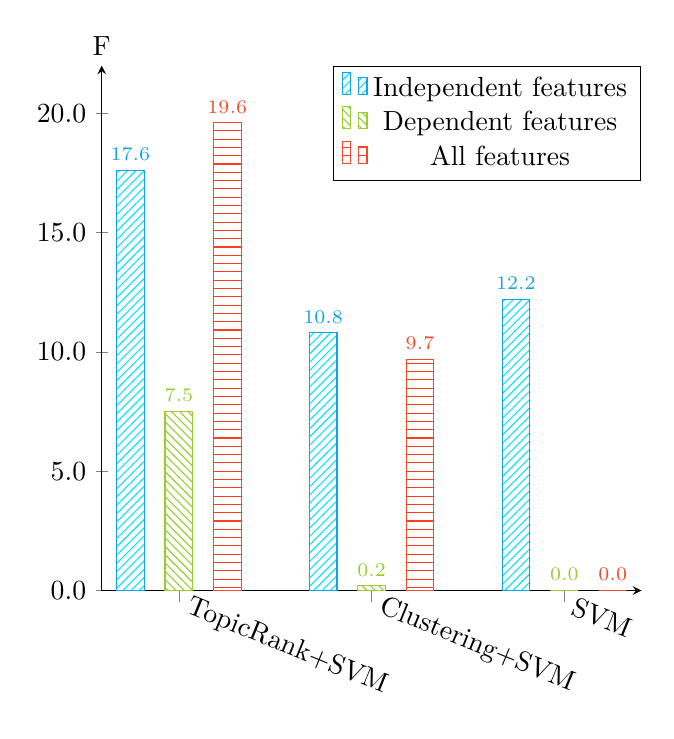
\begin{tikzpicture}%[scale=.75]
      \pgfkeys{/pgf/number format/.cd, fixed, fixed zerofill, precision=1}
      \begin{axis}[axis lines=left,
                   symbolic x coords={TopicRank+SVM, Clustering+SVM, SVM},
                   xtick=data,
                   enlarge x limits=0.2,
                   %x=.25\linewidth,
                   xticklabel style={anchor=west, rotate=-22.25},
                   nodes near coords,
                   nodes near coords align={vertical},
                   every node near coord/.append style={font=\scriptsize},
                   ytick={0.0, 5.0, 10.0, 15.0, 20.0, 25.0},
                   y=0.025\linewidth,
                   ymin=0.0,
                   ymax=22.0,
                   ybar=7.5pt,
                   ylabel=F,
                   ylabel style={at={(ticklabel* cs:1)},
                                 anchor=south,
                                 rotate=270},
                   legend style={at={(1.0, 1.0)},
                                 anchor=north east}]
        \addplot[Cerulean,
                 pattern=north east lines,
                 pattern color=Cerulean] coordinates{
          (SVM, 12.2)
          (Clustering+SVM, 10.8)
          (TopicRank+SVM, 17.6)
        };
        \addplot[YellowGreen,
                 pattern=north west lines,
                 pattern color=YellowGreen] coordinates{
          (SVM, 0.0)
          (Clustering+SVM, 0.2)
          (TopicRank+SVM, 7.5)
        };
        \addplot[RedOrange,
                 pattern=horizontal lines,
                 pattern color=RedOrange] coordinates{
          (SVM, 0.0)
          (Clustering+SVM, 9.7)
          (TopicRank+SVM, 19.6)
        };
        \legend{Independent features, Dependent features, All features}
      \end{axis}
    \end{tikzpicture}
    \caption{Performance of TopicRank+SVM$_{all}$ compared to derived baselines
             \label{fig:baseline_comparison}}
  \end{figure}

  Also, Table~\ref{tab:state_of_the_art_comparison} presents a comparison of
  TopicRank+SVM$_{all}$ with TopicRank, TopicRank's best possible performance
  (TopicRank$_{max}$) and common baselines of previous work. Results show that
  our method significantly improves TopicRank and significantly outperform
  TF-IDF and KEA, a robust supervised methods. However, the performance of
  TopicRank+SVM$_{all}$ is still very low compared to the best possible
  performance that could be achieved with TopicRank. The naivety of the
  clustering method TopicRank applies may introduce noise that dampens the
  performance. Future improvement should focus on a more efficient clustering of
  the candidates belonging to the same topic.
  \begin{table}[h]
    \centering
    \begin{tabular}{|r|rrr|}
      \hline
      Method & \multicolumn{1}{c}{P} & \multicolumn{1}{c}{R} & \multicolumn{1}{c|}{F}\\
      \hline
      KEA                   & 18.8\textcolor{white}{$^\dagger$} & 13.3\textcolor{white}{$^\dagger$} & 15.4\textcolor{white}{$^\dagger$}\\
      TF-IDF                & 13.2\textcolor{white}{$^\dagger$} & 8.9\textcolor{white}{$^\dagger$} & 10.5\textcolor{white}{$^\dagger$}\\
      TopicRank             & 14.9\textcolor{white}{$^\dagger$} & 10.3\textcolor{white}{$^\dagger$} & 12.1\textcolor{white}{$^\dagger$}\\
      TopicRank+SVM$_{all}$ & 24.2$^\dagger$ & 16.7$^\dagger$ & 19.6$^\dagger$\\
      \hline
      TopicRank$_{max}$     & 37.6\textcolor{white}{$^\dagger$} & 25.8\textcolor{white}{$^\dagger$} & 30.3\textcolor{white}{$^\dagger$}\\
      \hline
    \end{tabular}
    \caption{Performance of TopicRank+SVM$_{all}$ compared to previous work.
      $\dagger$ indicates improvement over KEA, TF-IDF and TopicRank at 0.001
      level using Student's t-test.
             \label{tab:state_of_the_art_comparison}}
  \end{table}

%\section{Error Analysis}
%\label{sec:error_analysis}


\section{Analyse d'erreurs}
\label{sec:analyse_d_erreurs}
  Dans cette section, nous proposons d'analyser les erreurs de TopicRank. Dans
  un premier temps, nous analysons les sujets que détecte TopicRank, puis dans
  un second temps, nous analysons les termes-clés de référence qui ne sont pas
  extraits par Topic\-Rank.

  \subsection{Analyse des sujets détectés}
  \label{subsec:analyse_des_sujets_générés}
    Dans cette section, nous analysons les groupements en sujets effectués par
    Topic\-Rank afin de déterminer quelles sont les principales causes
    d'erreurs.

    Nous observons des erreurs liées à la sélection des
    termes-clés candidats. Lors de cette étape, certaines unités textuelles sont
    sélectionnées comme candidats à cause d'erreurs commises lors de l'étiquetage
    grammatical. Ces erreurs concernent principalement la détection des
    prépositions composées et la détection des participes. Par exemple, dans la
    phrase \og{}[\dots] elles ne cessent de se développer à travers le monde et
    particulièrement dans les pays dits ``du sud'' [\dots]\fg{}\footnote{Exemple
    issu de l'article d'anthropologie \textit{Le marché parallèle du médicament
    en milieu rural au Sénégal} (\url{http://id.erudit.org/iderudit/014935ar})
    de la collection DEFT.}, le participe passé \og{}dits\fg{} est considéré
    comme un adjectif par l'outils MElt, ce qui entraîne la sélection erronée du
    termes-clés candidat \og{}pays dits\fg{}.

    Nous observons également de nombreuses erreurs lorsque les
    groupements sont déclenchés par un adjectif. Ce sont particulièrement les
    expansions nominales s'effectuant à gauche qui en sont la cause (p.~ex.
    \og{}même langue\fg{} groupé avec \og{}même représentation\fg{}). Parmi les
    expansions nominales s'effectuant à droite, les adjectifs relationnels sont
    moins sujets aux erreurs que les autres adjectifs. Notons tout de même que
    lorsque ces adjectifs sont liés au contexte général du document, ils sont
    très fréquemment utilisés et beaucoup de candidats les contenant sont
    groupés par erreur (p.~ex. \og{}forces économiques\fg{} peut être groupé 
    avec \og{}délabrement économique\fg{} dans un document en économie). Outres
    ces groupements erronés, nous observons aussi de mauvais groupements lorsque
    les candidats ne contiennent que très peu de mots. Pour les candidats de
    deux mots, il ne suffit que d'un seul mot en commun pour les grouper. Ces
    candidats étant très fréquents, ils sont la cause de nombreuses erreurs.

  \subsection{Analyse des faux négatifs}
  \label{subsec:analyse_faux_négatifs}
    Dans cette section, nous analysons les termes-clés de référence qui n'ont
    pas été extraits par TopicRank. Plus particulièrement, nous nous intéressons
    à ceux qui sont présents dans les 10 sujets jugés les plus importants de
    chaque document, mais qui n'ont pas été sélectionnés pour les représenter.
    Nous observons deux sources d'erreurs.

    La première source d'erreurs est le groupement en sujets. Lorsqu'un sujet
    détecté contient en réalité des termes-clés candidats représentant des
    sujets différents, la stratégie de sélection du meilleur terme-clé dans le
    sujet parvient à sélectionner le terme-clé correct dans certains cas, mais
    elle échoue parfois.

    La seconde source d'erreurs est la spécialisation des termes-clés de
    référence. Nous observons deux problèmes de sous- et sur-spécialisation de
    certains termes-clés extraits vis-à-vis des termes-clés de référence. Dans
    le cas de la sous-spécialisation, nous pouvons citer, par exemple,
    \og{}papillons\fg{} qui est extrait à la place de \og{}papillons
    mutants\fg{}\footnote{Exemple issue de l'article journalistique
    \textit{Fukushima fait muter les papillons}
    (\url{http://fr.wikinews.org/w/index.php?oldid=432477}) de la collection
    WikiNews.}. Bien que ce problème de sous-spécialisation soit identifié,
    l'existance du problème inverse le rend plus difficile à résoudre. Dans le
    cas de la sur-spécialisation, nous pouvons citer, par exemple, \og{}député
    Antoni Pastor\fg{} qui est extrait à la place de \og{}Antoni
    Pastor\fg{}\footnote{Exemple issu de l'article journalistique \textit{Îles
    Baléares : le Parti populaire exclut le député Antoni Pastor pour avoir
    défendu la langue catalane}
    (\url{http://fr.wikinews.org/w/index.php?oldid=479948}) de la collection
    WikiNews.}. La raison principale de ce problème est l'aspect libre de
    l'annotation manuelle des termes-clés. Toutefois, privilégier les
    modifications adjectivales (p.~ex. \og{}mutants\fg{}) et, au contraire,
    éviter les modifications nominales (p.~ex. \og{}député\fg{}) semble être une
    hypothèse à vérifier.


\section{Conclusion et perspectives}
\label{sec:conclusion_et_perspectives}
  Dans cet article, nous nous intéressons à la tâche d'extraction automatique de
  termes-clés dans les documents scientifiques et émettons l'hypothèse que sa
  difficulté est variable selon la discipline des documents traités. Pour
  vérifier cette hypothèse, nous disposons de notices bibliographiques réparties
  dans cinq disciplines (archéologie, linguistique, sciences de l'information,
  psychologie et chimie) auxquelles nous appliquons six systèmes d'extractions
  automatique de termes-clés différents. En comparant les termes-clés extraits
  par chaque système avec les termes-clés de référence assignés aux notices dans
  des conditions réels d'indexation, notre hypothèse se vérifie et nous
  observons l'échelle suivante (de la discipline la plus facile à la plus
  difficile)~:
  \begin{enumerate*}
    \item{Archéologie~;}
    \item{Linguistique~;}
    \item{Sciences de l'information~;}
    \item{Psychologie~;}
    \item{Chimie.}
  \end{enumerate*}

  À l'issue de nos expériences et de nos observations du contenu des notices,
  nous constatons deux facteurs ayant un impact sur la difficulté de la tâche
  d'extraction automatique de termes-clés. Tout d'abord, nous observons que
  l'organisation du résumé peut aider l'extraction de termes-clés. Un résumé
  riche en explications et en mises en relations des différents concepts est
  moins difficile à traiter qu'un résumé énumératif pauvre en explications.
  Ensuite, le vocabulaire utilisé dans une discipline peut influer sur la
  difficulté à extraire les termes-clés des documents de cette discipline. Si le
  vocabulaire spécifique contient des composés syntagmatiques dont certains
  éléments sont courants dans la discipline, alors il peut être plus difficile
  d'extraire les termes-clés des documents de cette discipline.

  Des deux facteurs identifiés émergent plusieurs perspectives de travaux
  futurs. Il peut être intéressant d'analyser le discours des documents afin de
  mesurer, en amont, le degré de difficulté de l'extraction de termes-clés. Avec
  une telle connaissance, nous pourrions proposer une méthode capable de
  s'adapter au degré de difficulté en ajustant automatiquement son paramètrage.
  Cependant, l'analyse que nous proposons dans cet article se fonde uniquement
  sur le contenu de notices appartenant à cinq disciplines. Il serait pertinent
  d'étendre cette analyse au contenu intégral des documents scientifiques, ainsi
  que d'élargir le panel de disciplines utilisées dans ce travail, afin
  d'établir des catégories de discplines plus ou moins difficiles à traiter
  (p.~ex. la chimie fait partie des disciplines expérimentales, qui sont
  difficiles à traiter). Nous oberservons aussi que le vocabulaire utilisé dans
  une discipline, en particulier celui utilisé pour les termes-clés, peut rendre
  la tâche d'extraction automatique de termes-clés plus difficile. Il est donc
  important de bénéficier de resources telles que des thésaurus pour permettre à
  une méthode d'extraction de termes-clés de s'adapter au domaine. Pour
  TopicRank, par exemple, avoir connaissance de la terminologie utilisée dans
  une discipline peut améliorer le choix du terme-clé le plus représentatif d'un
  sujet. Enfin, il serait intéressant de penser la tâche d'extraction de
  termes-clés comme une tâche d'extraction d'information pour le remplissage
  d'un formulaire. En archéologie, par exemple, il pourrait s'agir d'extraire
  les informations géographiques (pays, régions, etc.), chronologiques (période,
  culture, etc.), ou encore environnementales (animaux, végétaux, etc.).



\acknowledgements{
  Ce travail a bénéficié d'une aide de l'Agence nationale de la recherche
  portant la référence (ANR-12-CORD-0029).
}

\bibliography{./biblio}

\end{document}

